%%%%%%%%%%%%%%%%%%%%%%%%%%%%%%%%%%%
%%  Einführung
%%%%%%%%%%%%%%%%%%%%%%%%%%%%%%%%%%%
\section*{Einführung ins Thema}

Die Wetterstation Arbon wurde 2005 als Lehrlingsarbeit des Berufsbildungszentrums Arbon auf Initiative der Technischen Gesellschaft Arbon (TGA) aufgebaut und in Betrieb genommen. Sie besteht aus mehreren Wettersensoren und einer Webcam, die auf einer Plattform auf dem See draussen montiert sind. Die Messwerte werden auf der Webseite\footnote{ \url{https://www.wetter-arbon.ch }}  der Wetterstation Arbon angezeigt.

\begin{figure}[h!]
	\centering
	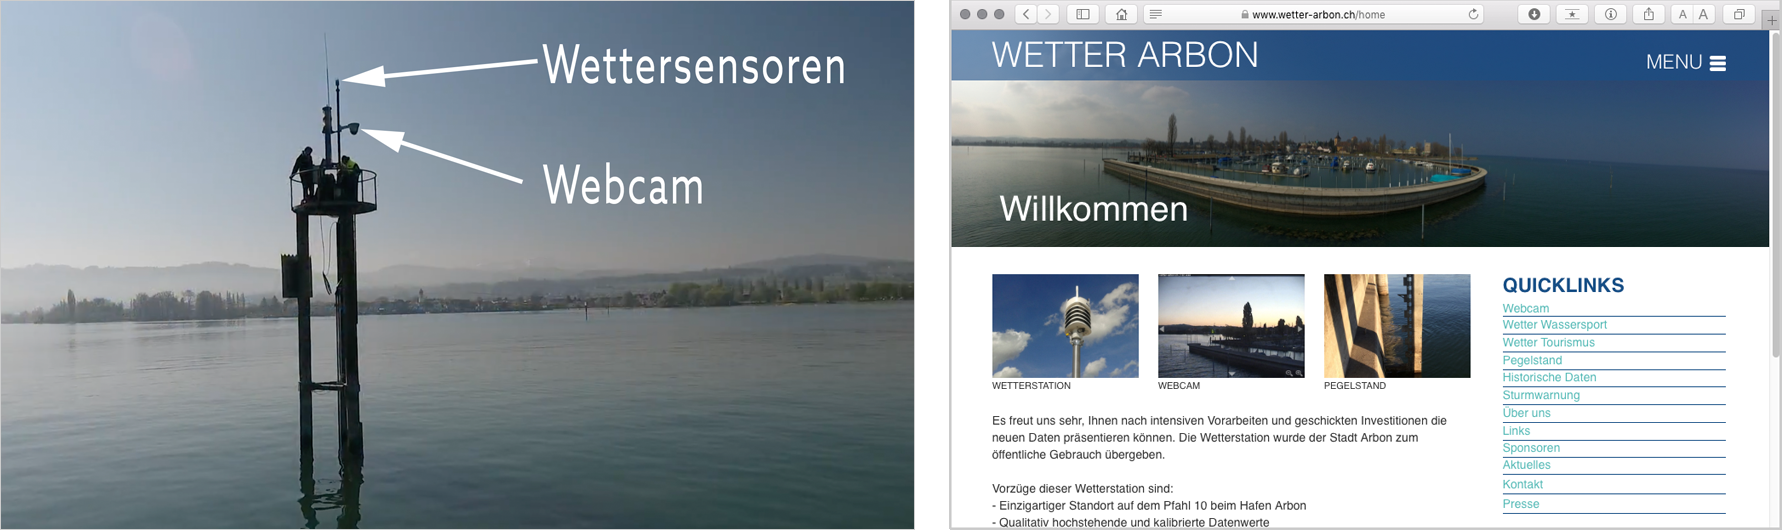
\includegraphics[width=1\linewidth]{img/kombi}
	\caption{Installation und Webseite der Wetterstation Arbon}
	\label{img:wetterstation}
\end{figure}

Was damals modern war, ist heute veraltet. Sowohl auf der Hardwareseite, als auch auf der Webseite gibt es diverses Reparatur- beziehungsweise Modernisierungspotential. Während des Fachmoduls führten wir eine Ist-Aufnahme der Wetterstation Arbon durch. Im Fokus lag sowohl die Hardware als auch die Software. Der Übersicht halber und damit wir die Arbeiten besser untereinander aufteilen konnten, haben wir die Themen in die vier Blöcke:  Webseite, Datenbank, Sensoren und Webcam unterteilt. (Abb. \ref{img:module})

\vspace{5mm} %5mm vertical space

\begin{figure}[h!]
	\centering
	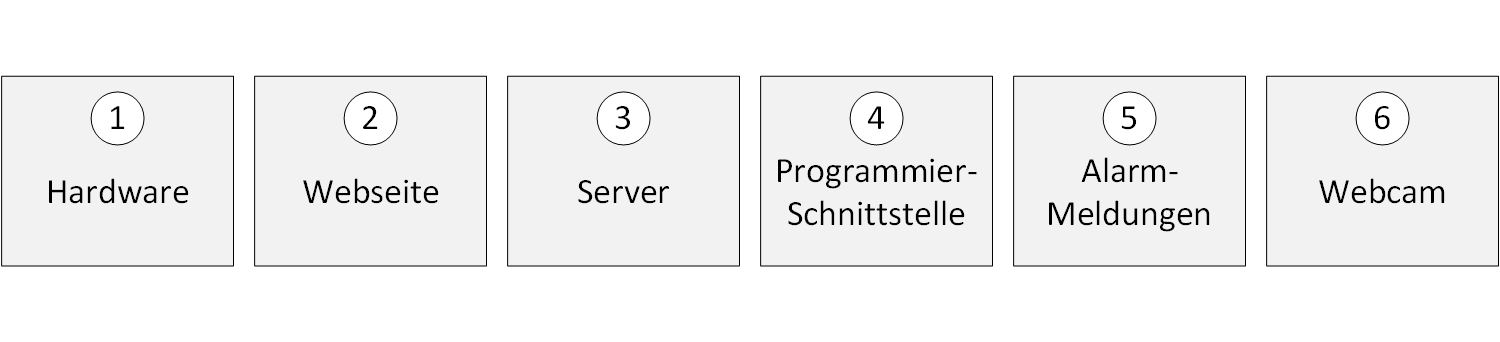
\includegraphics[width=0.8\linewidth]{img/module}
	\caption{Aufteilung in Arbeitsblöcke}
	\label{img:module}
\end{figure}

Bei jedem Block führten wir eine Analyse der der ist-Situation durch und identifizierten die vorhandenen Probleme. 
Dieser Bericht zeigt jeweils pro Block auf, wo die Problemstellen liegen, wie diese behoben werden können und was die Anforderungen an die Lösung ist.

\newpage

%% Beispiel für die Einbindung von Grafiken
%\Diskussionspunkt{Beispiel für eine Bildintegration inkl. Referenz darauf:}
%\begin{figure}[h]
%	\centering
%	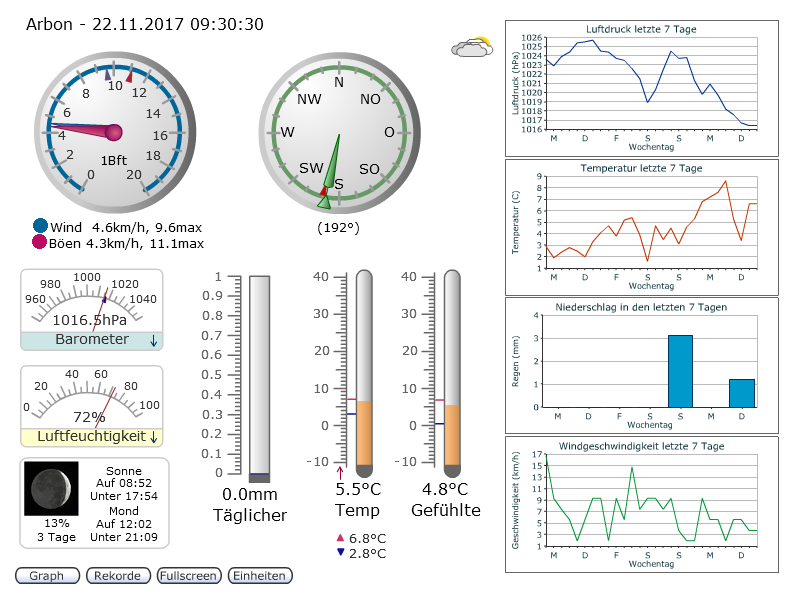
\includegraphics[width=0.6\linewidth]{img/grafik}
%	\caption{eine Grafik ohne Sinn und Verstand}
%	\label{img:grafik-dummy}
%\end{figure}

%\ref{img:dummy} auf Seite \pageref{img:grafik-dummy} 
